\section{MATERIAIS E MÉTODOS}

Iniciou-se a parte prática com a construção de um protótipo capaz de executar consultas SQL, coletar informações sobre essas execuções e apresentar possíveis pontos de atenção. O estudo foi realizado em um ambiente controlado, com dados fictícios, para que os testes não interferissem em um sistema real.

O trabalho foi organizado em seis etapas. Primeiro, construiu-se o banco experimental. Depois, geraram-se e carregaram-se os dados. Na terceira etapa, executou-se um conjunto de consultas para formar um histórico. Na quarta, coletaram-se as estatísticas e selecionaram-se as consultas mais relevantes. Na quinta, analisaram-se os planos de execução. Por fim, comparou-se uma alteração de consulta e verificou-se seu resultado. A Figura~\ref{fig:fluxo-simples} apresenta esse processo.

\begin{figure}[H]
\centering
\caption{Etapas da solução desenvolvida}
\label{fig:fluxo-simples}
\begin{tikzpicture}[
etapa/.style={rectangle,draw=black,rounded corners,align=center,
  text width=10.5cm,minimum height=0.78cm,font=\small},
seta/.style={-{Latex[length=2mm]},thick},node distance=0.35cm]
\node[etapa] (e1) {1. Construção do banco experimental};
\node[etapa,below=of e1] (e2) {2. Geração e carregamento dos dados fictícios};
\node[etapa,below=of e2] (e3) {3. Execução das consultas e formação do histórico};
\node[etapa,below=of e3] (e4) {4. Coleta e classificação das estatísticas};
\node[etapa,below=of e4] (e5) {5. Análise preventiva dos planos de execução};
\node[etapa,below=of e5] (e6) {6. Comparação e validação de uma alteração};
\draw[seta] (e1) -- (e2);
\draw[seta] (e2) -- (e3);
\draw[seta] (e3) -- (e4);
\draw[seta] (e4) -- (e5);
\draw[seta] (e5) -- (e6);
\end{tikzpicture}
\fonteautor
\end{figure}

\subsection{Ambiente de desenvolvimento}

Na primeira rodada experimental foram utilizados PostgreSQL 18.1, Python 3.14.3 e Psycopg 3.3.6 em Windows de 64 bits. O PostgreSQL armazenou os dados, executou as consultas e forneceu seus planos. O Python foi usado para gerar os dados, organizar os testes e apresentar os resultados. O Psycopg fez a comunicação entre o programa e o banco. O DBeaver auxiliou na administração e na conferência das tabelas.

Após a formatação do computador, o projeto foi preparado novamente com PostgreSQL 18.6 e Python 3.14.7. Nessa verificação, o computador possuía processador AMD Ryzen 5 5600X, aproximadamente 32~GB de memória RAM, SSD de 2~TB e Windows 11 Pro. Os resultados da primeira rodada foram mantidos separados dessa verificação posterior, pois mudanças no ambiente podem influenciar os tempos.

Os arquivos foram organizados em pastas para os scripts SQL, os programas Python, a documentação e os resultados. Também foi criado um ambiente virtual Python para registrar as dependências do projeto e facilitar uma nova instalação.

\subsection{Banco experimental e geração dos dados}

Criou-se o banco \texttt{tcc\_sql\_optimizer} com cinco tabelas: clientes, produtos, pedidos, itens de pedido e pagamentos. Um cliente pode realizar vários pedidos; cada pedido pode possuir vários itens; cada item associa um produto ao pedido; e o pagamento registra a situação financeira do pedido. Essa estrutura representa operações comuns de uma loja e permite testar filtros, junções, agrupamentos e ordenações.

Todas as tabelas receberam chave primária. Também foram definidas chaves estrangeiras para preservar os relacionamentos. O e-mail do cliente foi definido como único, criando um índice que depois pôde ser utilizado no teste de busca por e-mail. Não foram acrescentados índices apenas para favorecer as consultas do experimento.

A Figura~\ref{fig:modelo-simples} resume os relacionamentos. Ela também ajuda a compreender por que algumas consultas precisam juntar várias tabelas: para chegar dos dados de um cliente aos produtos comprados, por exemplo, o banco passa pelos pedidos e pelos itens.

\begin{figure}[H]
\centering
\caption{Relacionamentos principais do banco experimental}
\label{fig:modelo-simples}
\begin{tikzpicture}[
tabela/.style={rectangle,draw=black,rounded corners,align=center,
  minimum width=2.5cm,minimum height=0.8cm,font=\small},
rel/.style={-{Latex[length=2mm]},thick}]
\node[tabela] (clientes) at (0,1.5) {Clientes};
\node[tabela] (pedidos) at (4,1.5) {Pedidos};
\node[tabela] (itens) at (8,1.5) {Itens de pedido};
\node[tabela] (produtos) at (8,0) {Produtos};
\node[tabela] (pagamentos) at (4,0) {Pagamentos};
\draw[rel] (clientes) -- node[above,font=\footnotesize]{realiza} (pedidos);
\draw[rel] (pedidos) -- node[above,font=\footnotesize]{possui} (itens);
\draw[rel] (produtos) -- node[right,font=\footnotesize]{é referenciado} (itens);
\draw[rel] (pedidos) -- node[right,font=\footnotesize]{gera} (pagamentos);
\end{tikzpicture}
\fonteautor
\end{figure}

O programa de geração criou os volumes apresentados na Tabela~\ref{tab:volumes-simples}. As quantidades não vieram de uma empresa real. Elas foram escolhidas para combinar tabelas pequenas e grandes, produzir consultas rápidas e lentas e tornar visível a diferença entre uma leitura direcionada e uma leitura de muitos registros.

\begin{table}[H]
\centering
\caption{Volume do banco experimental}
\label{tab:volumes-simples}
\begin{tabular}{lr}
\toprule
\textbf{Tabela} & \textbf{Quantidade de registros} \\
\midrule
Clientes & 100.000 \\
Produtos & 50.000 \\
Pedidos & 1.000.000 \\
Itens de pedido & 2.498.714 \\
Pagamentos & 1.000.000 \\
\midrule
\textbf{Total} & \textbf{4.648.714} \\
\bottomrule
\end{tabular}
\fonteautor
\end{table}

Os dados incluíram diferentes estados, preços, datas, situações de pedido e frequências de compra. A distribuição foi controlada para gerar casos variados, mas não buscou reproduzir o comportamento de uma empresa específica. Depois da carga, utilizou-se o comando \texttt{ANALYZE} para que o PostgreSQL atualizasse as informações usadas na criação dos planos.

\subsection{Consultas e execução da carga}

Foram elaboradas 12 consultas SQL. Elas receberam nomes de Q01 a Q12 apenas para facilitar a organização do estudo. O conjunto incluiu filtros simples, junções, agrupamentos, ordenações, subconsultas e consultas que retornam muitos registros. A Tabela~\ref{tab:consultas-simples} resume a carga executada.

\begin{table}[H]
\centering
\caption{Consultas utilizadas no experimento}
\label{tab:consultas-simples}
\small
\begin{tabularx}{\textwidth}{c r Y}
\toprule
\textbf{Consulta} & \textbf{Chamadas} & \textbf{Objetivo principal} \\
\midrule
Q01 & 500 & Buscar um cliente pela chave primária. \\
Q02 & 100 & Filtrar e ordenar produtos. \\
Q03 & 60 & Consultar pedidos de um cliente. \\
Q04 & 20 & Listar pedidos cancelados. \\
Q05 & 15 & Buscar pedidos de um ano e os respectivos clientes. \\
Q06 & 10 & Agrupar dados das cinco tabelas. \\
Q07 & 8 & Somar pedidos por mês. \\
Q08 & 6 & Ordenar pedidos de maior valor. \\
Q09 & 5 & Buscar cliente aplicando uma função ao e-mail. \\
Q10 & 3 & Buscar pedidos acima do valor médio. \\
Q11 & 2 & Contar pedidos por cliente. \\
Q12 & 1 & Ler todos os itens de pedido. \\
\midrule
\textbf{Total} & \textbf{730} & \textbf{Chamadas executadas.} \\
\bottomrule
\end{tabularx}
\fonteautor
\end{table}

As quantidades foram definidas para criar três situações fáceis de comparar: uma consulta muito frequente, consultas intermediárias e consultas pouco frequentes que processam muitos dados. Antes da carga completa, executou-se cada consulta uma vez para verificar seu funcionamento. Em seguida, realizaram-se as 730 chamadas com valores de entrada fixos. Não foram simulados vários usuários ao mesmo tempo.

\subsection{Coleta e classificação das consultas}

A coleta utilizou a extensão \texttt{pg\_stat\_statements}, que mantém estatísticas acumuladas das consultas executadas \cite{postgresql2026pgstat}. Para cada consulta, foram observados principalmente o número de chamadas, o tempo total, o tempo médio e a quantidade de linhas retornadas.

Essas medidas respondem a perguntas diferentes. O tempo total mostra onde o banco gastou mais tempo no conjunto da carga. O tempo médio mostra quanto uma chamada costuma demorar. A frequência mostra quais consultas foram executadas mais vezes. Por isso, uma consulta frequente não é necessariamente a mais lenta, e uma consulta executada apenas uma vez pode retornar muitos dados.

A Tabela~\ref{tab:metricas-simples} apresenta uma leitura resumida dessas informações. Não há uma fórmula de classificação que determine sozinha qual consulta deve ser alterada. As métricas funcionam como pontos de partida para selecionar o que será investigado.

\begin{table}[H]
\centering
\caption{Significado das principais métricas}
\label{tab:metricas-simples}
\begin{tabularx}{\textwidth}{l Y Y}
\toprule
\textbf{Métrica} & \textbf{O que informa} & \textbf{Como foi utilizada} \\
\midrule
Chamadas & Quantas vezes a consulta apareceu. & Identificar consultas frequentes. \\
Tempo total & Tempo somado de todas as chamadas. & Localizar onde o banco acumulou mais trabalho. \\
Tempo médio & Duração média de uma chamada. & Encontrar consultas individualmente demoradas. \\
Linhas & Quantidade de registros retornados. & Evitar comparar consultas de volumes muito diferentes como se fossem iguais. \\
\bottomrule
\end{tabularx}
\fonteautor
\end{table}

O coletor relacionou as estatísticas com as consultas Q01 a Q12 e exportou os resultados para arquivos CSV e JSON. Esses arquivos facilitaram a conferência e permitiram que a interface apresentasse as informações sem exigir a leitura direta das tabelas internas do PostgreSQL.

\subsection{Análise preventiva dos planos de execução}

O analisador recebe uma instrução \texttt{SELECT} e solicita ao PostgreSQL apenas o plano estimado, por meio de \texttt{EXPLAIN} sem \texttt{ANALYZE}. Assim, a consulta candidata não é executada durante essa análise \cite{postgresql2026explain}. O plano mostra como o banco pretende localizar, combinar e ordenar os dados.

O protótipo procura sinais simples que merecem atenção: uso de \texttt{SELECT *}, leitura sequencial de uma tabela grande, função aplicada sobre uma coluna usada no filtro, retorno de muitas linhas e diferença elevada entre a quantidade prevista no plano e a quantidade observada no histórico. Cada sinal gera uma explicação e uma sugestão de investigação.

Os níveis baixo, médio e alto servem somente para ordenar os casos. Eles não provam que uma consulta está errada e não representam tempo de execução. A ferramenta também não cria índices nem altera comandos automaticamente. A decisão depende da análise do desenvolvedor e de um teste posterior.

\subsection{Comparação e validação}

Selecionaram-se dois casos para demonstração. Na consulta de pedidos por ano, comparou-se o plano da forma original, que aplicava uma função sobre a data, com o plano de uma alternativa que utilizava um intervalo de datas. Essa comparação foi apenas preventiva: as consultas não foram executadas para medir qual delas seria mais rápida.

Na busca por e-mail, comparou-se a aplicação de \texttt{LOWER} sobre a coluna com uma comparação direta. A alternativa poderia usar o índice já existente. Como todos os e-mails da base foram armazenados em letras minúsculas, verificou-se se as duas formas retornavam o mesmo registro. Depois, cada versão foi executada 100 vezes. O programa comparou os tempos médios informados pelo PostgreSQL. O percentual apresentado nos resultados foi calculado automaticamente a partir da diferença entre essas duas médias, sem exigir uma fórmula específica do usuário da ferramenta.

\subsection{Interface do protótipo}

Desenvolveu-se uma interface web local para facilitar a apresentação do projeto. A tela inicial resume a quantidade de consultas, o número de chamadas e o tempo acumulado. Outras telas permitem escolher uma consulta, visualizar seu histórico, analisar o plano estimado e comparar a versão original com uma alternativa.

A interface informa quando uma operação é apenas preventiva e quando houve uma medição real. Também impede comandos de alteração, como \texttt{INSERT}, \texttt{UPDATE} e \texttt{DELETE}, pois o objetivo do protótipo é analisar instruções de leitura. Foram realizados testes de funcionamento das principais rotas e da comunicação com o banco.

\section{RESULTADOS E DISCUSSÃO}

Os resultados foram organizados de acordo com as etapas descritas na metodologia. Primeiro, apresentam-se as estatísticas da carga. Depois, discutem-se duas consultas selecionadas e a interface criada para tornar a análise mais visual.

\subsection{Resultados da carga de consultas}

O teste inicial executou as 12 consultas sem erros. Na carga completa, foram realizadas 730 chamadas. O programa Python registrou aproximadamente 103,2 segundos para essa rodada. O valor inclui o tempo necessário para o programa receber os resultados, enquanto as estatísticas internas do PostgreSQL registraram aproximadamente 102,6 segundos de execução no servidor.

Os três critérios de classificação destacaram consultas diferentes, como mostra a Tabela~\ref{tab:destaques-simples}.

\begin{table}[H]
\centering
\caption{Consultas destacadas pelas estatísticas}
\label{tab:destaques-simples}
\begin{tabularx}{\textwidth}{c r r r Y}
\toprule
\textbf{Consulta} & \textbf{Chamadas} & \textbf{Total (ms)} & \textbf{Média (ms)} & \textbf{Motivo do destaque} \\
\midrule
Q05 & 15 & 42.472,08 & 2.831,47 & Maior tempo acumulado. \\
Q12 & 1 & 6.795,63 & 6.795,63 & Maior duração em uma chamada. \\
Q01 & 500 & 9,25 & 0,02 & Maior frequência. \\
\bottomrule
\end{tabularx}
\fonteautor
\end{table}

A Q05 foi o principal caso para investigação porque concentrou o maior tempo total. A Q12 apresentou o maior tempo por chamada, mas foi executada apenas uma vez e retornou 2.498.714 linhas. Portanto, esse valor não deve ser tratado como uma média representativa. A Q01 foi executada 500 vezes, porém continuou rápida por buscar um cliente pela chave primária. Esses resultados mostram por que frequência, tempo e volume precisam ser observados em conjunto.

\subsection{Consulta de pedidos por ano}

A Q05 seleciona pedidos de 2026 e os dados dos respectivos clientes. Na forma original, o filtro extrai o ano de cada data:

\begin{lstlisting}[language=SQL]
SELECT *
FROM public.pedidos p
JOIN public.clientes c ON c.id = p.cliente_id
WHERE EXTRACT(YEAR FROM p.data_pedido) = 2026;
\end{lstlisting}

O plano estimou 5.000 linhas, enquanto o histórico indicou uma média próxima de 499.676 linhas por execução. Em outras palavras, a consulta normalmente retornou quase 100 vezes mais linhas do que o plano previa. O analisador também identificou a seleção de todas as colunas, a leitura sequencial da tabela de pedidos e a função aplicada sobre a data.

Preparou-se uma alternativa que compara a coluna diretamente com o início e o fim do ano:

\begin{lstlisting}[language=SQL]
WHERE p.data_pedido >= TIMESTAMP '2026-01-01 00:00:00'
  AND p.data_pedido <  TIMESTAMP '2027-01-01 00:00:00'
\end{lstlisting}

No novo plano, a previsão passou para aproximadamente 499.434 linhas, valor muito mais próximo do histórico. Isso mostra que a escrita do filtro ajudou o banco a prever melhor o volume de saída. Entretanto, não se afirmou que a alternativa ficou mais rápida, pois ela não foi executada nessa comparação. O resultado foi mantido como uma recomendação para teste posterior.

\begin{table}[H]
\centering
\caption{Resumo da comparação da consulta de pedidos por ano}
\label{tab:ano-resumo}
\begin{tabularx}{\textwidth}{l Y Y}
\toprule
\textbf{Aspecto} & \textbf{Forma original} & \textbf{Alternativa} \\
\midrule
Filtro & Extração do ano da data. & Comparação com início e fim do ano. \\
Linhas previstas & 5.000 & Aproximadamente 499.434 \\
Referência histórica & \multicolumn{2}{c}{Aproximadamente 499.676 linhas por chamada.} \\
Conclusão & Previsão distante do histórico. & Previsão mais próxima; tempo não medido. \\
\bottomrule
\end{tabularx}
\fonteautor
\end{table}

\subsection{Busca por e-mail}

A Q09 aplicava a função \texttt{LOWER} sobre a coluna de e-mail. Mesmo existindo um índice nessa coluna, o plano original previa uma leitura sequencial dos 100.000 clientes. A alternativa comparou o e-mail diretamente com o valor já normalizado em letras minúsculas, permitindo a utilização do índice.

\begin{lstlisting}[language=SQL]
-- Forma original
WHERE LOWER(email) = 'cliente123@example.com';

-- Alternativa avaliada
WHERE email = 'cliente123@example.com';
\end{lstlisting}

As duas formas retornaram o mesmo cliente nos testes. Em 100 chamadas de cada versão, o tempo médio informado pelo servidor caiu de 26,33 milissegundos para 0,0303 milissegundo. Isso correspondeu a uma redução aproximada de 99,88\% nas condições do experimento. O resultado não significa que toda função deva ser removida de um filtro. Nesse caso específico, a mudança foi válida porque os e-mails da base já estavam armazenados em letras minúsculas.

\begin{table}[H]
\centering
\caption{Resumo da comparação da busca por e-mail}
\label{tab:email-resumo}
\begin{tabularx}{\textwidth}{l Y Y}
\toprule
\textbf{Aspecto} & \textbf{Forma original} & \textbf{Alternativa} \\
\midrule
Comparação & Função \texttt{LOWER} sobre a coluna. & Comparação direta com o e-mail. \\
Plano & Leitura sequencial dos clientes. & Uso do índice existente. \\
Tempo médio & 26,33 ms & 0,0303 ms \\
Resultado & \multicolumn{2}{c}{Mesmo cliente retornado nos testes realizados.} \\
\bottomrule
\end{tabularx}
\fonteautor
\end{table}

A comparação também mostrou uma diferença importante entre previsão e medição. Para a consulta por ano, houve somente análise do plano. Para a busca por e-mail, houve comparação do resultado e execução repetida das duas versões. Somente o segundo caso permitiu apresentar uma redução de tempo medida.

\subsection{Apresentação visual}

A interface reuniu o histórico, os planos e as sugestões em uma apresentação mais simples. A Figura~\ref{fig:interface-simples} mostra a visão geral, que apresenta as quantidades do experimento e as consultas com maior tempo acumulado.

\begin{figure}[H]
\centering
\caption{Visão geral da interface web}
\label{fig:interface-simples}
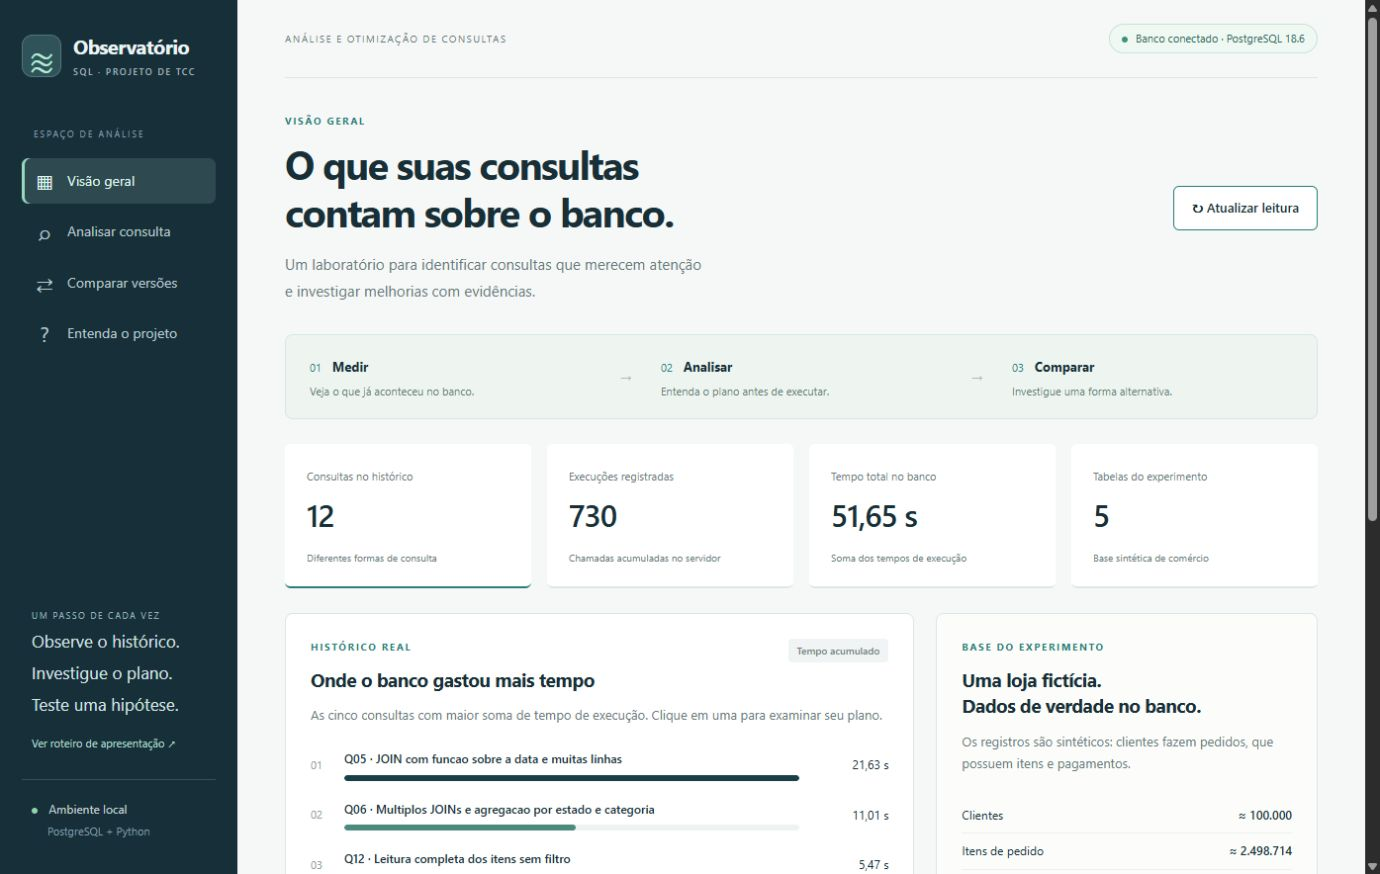
\includegraphics[width=0.88\textwidth]{images/interface.png}
\fonteautor
\end{figure}

Na tela de análise, o usuário pode escolher um exemplo ou colar uma instrução \texttt{SELECT}. O sistema mostra o plano estimado, os sinais encontrados e uma explicação de cada sugestão. Na tela de comparação, a versão original e a alternativa são apresentadas lado a lado. Essa organização permite demonstrar o funcionamento do projeto sem depender apenas do terminal.

Uma verificação posterior confirmou a carga com 730 chamadas e a leitura das 12 consultas pela interface. Também foram testados a rejeição de SQL inválido, o caso de uma consulta sem histórico e a análise sem execução da consulta candidata. Esses testes verificaram o funcionamento do protótipo, mas não correspondem a uma avaliação de usabilidade com participantes.

\subsection{Limitações dos resultados}

O estudo utilizou dados fictícios, valores de filtro fixos e quantidades de chamadas definidas para o experimento. Por isso, os resultados não permitem afirmar que a mesma classificação ocorreria em uma empresa real. Além disso, os tempos podem variar conforme o computador, o uso de memória e outros programas em execução.

A Q12 teve somente uma chamada e, portanto, seu tempo não representa várias observações. A consulta por ano teve apenas uma comparação preventiva de planos. Já o ganho da busca por e-mail depende de os endereços estarem armazenados em letras minúsculas. Essas condições precisam ser mencionadas ao apresentar os resultados.

O protótipo foi desenvolvido para PostgreSQL e uso local. Sua aplicação em produção exigiria novos testes, controle de permissões e avaliação com diferentes consultas e volumes de dados.

\section{CONCLUSÃO}

Este trabalho desenvolveu um processo para identificar e analisar consultas SQL com possíveis problemas de desempenho. A solução combinou estatísticas históricas do PostgreSQL, planos de execução, regras de análise e uma interface web.

Os resultados mostraram que tempo total, tempo médio e frequência destacam situações diferentes. A consulta de pedidos por ano apresentou o maior tempo acumulado, a leitura de todos os itens teve a maior duração em uma única chamada e a busca pela chave primária foi a mais frequente. Assim, uma consulta não deve ser escolhida para análise com base em apenas um número.

Na consulta de pedidos por ano, a alteração do filtro aproximou a quantidade prevista da quantidade observada no histórico, mas não foi medida como otimização. Na busca por e-mail, a comparação direta permitiu o uso do índice existente e reduziu o tempo médio do servidor de 26,33 para 0,0303 milissegundo, mantendo o mesmo resultado nas condições avaliadas.

Concluiu-se que a combinação de histórico e planos pode ajudar a localizar consultas relevantes e explicar por que uma alteração merece ser testada. A ferramenta não modifica automaticamente o banco e não substitui a validação. Sua função é organizar as evidências e apoiar a decisão do desenvolvedor.

Como continuidade, podem ser realizados novos testes com diferentes valores de entrada, mais repetições e outros bancos de dados. Também pode ser feita uma avaliação da interface com usuários para verificar se as explicações são suficientemente claras.
